\begin{figure}[p]
\centering
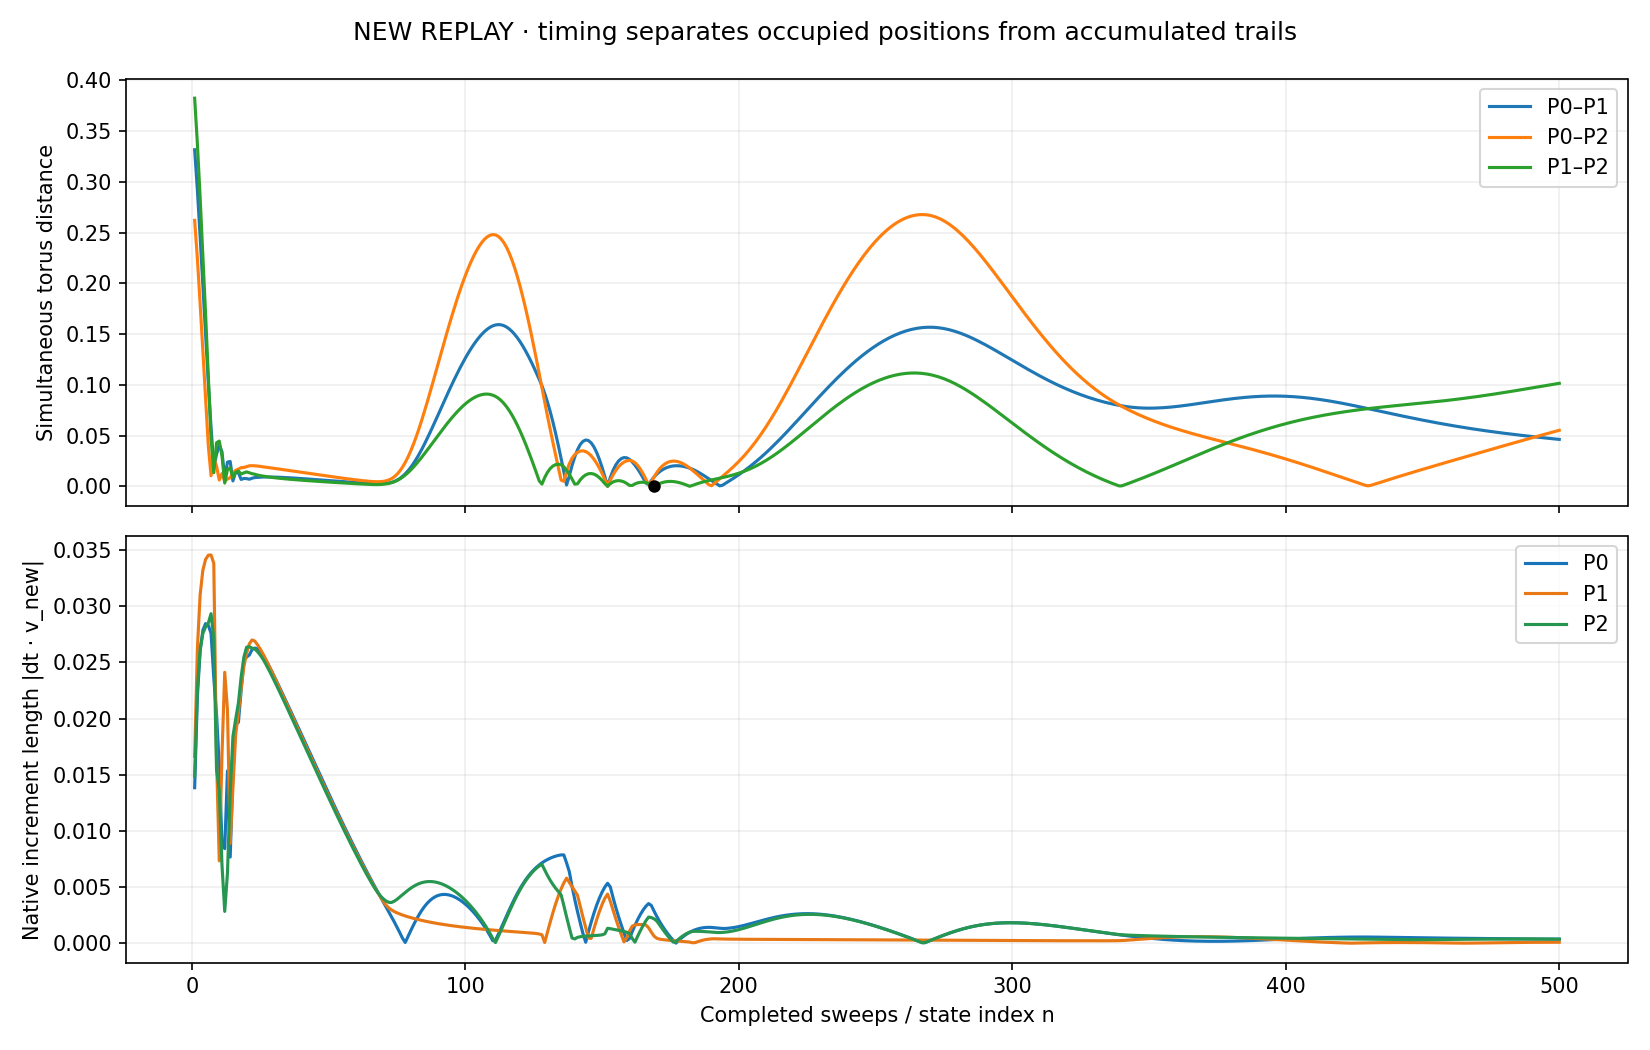
\includegraphics[width=\linewidth,height=0.70\textheight,keepaspectratio]{figures/F05_0.png}
\caption[Separation and increments across the reproduced record]{DERIVED from the accepted REPRODUCED S01 record. The upper panel measures simultaneous periodic pair separation at sweep boundaries; the lower measures native update lengths. The horizontal axis is completed-sweep chronology, not historical movie time. Repeated approaches and smaller late movement do not establish an asymptotic limit. Reused without recalculation. \cite{replay01}}
\label{fig:F05}
\end{figure}
